% Adapted to the supplied Chinese report template; XeLaTeX.
\documentclass[UTF8,punct,fontset=none]{ctexart}
\usepackage{fontspec,xeCJK}
\setmainfont{TeX Gyre Termes}
\setCJKmainfont[AutoFakeBold=true]{FandolKai-Regular.otf}
\newCJKfontfamily\zhkai[AutoFakeBold=true]{FandolKai-Regular.otf}
\newfontfamily\enkai{TeX Gyre Termes}
\setCJKsansfont{FandolHei-Regular.otf}
\setCJKmonofont{FandolFang-Regular.otf}
\usepackage{amsmath,amssymb,cases,cite,graphicx}
\usepackage[a4paper,left=2.50cm,right=2.50cm,top=2.70cm,bottom=2.56cm]{geometry}
\usepackage{fancyhdr,tabularx,booktabs,longtable,array,makecell,enumitem}
\usepackage{pdfpages,pdflscape,tikz,pgfplots,xcolor,float,caption}
\usetikzlibrary{arrows.meta,positioning,fit,calc,backgrounds}
\pgfplotsset{compat=1.18}
\usepackage[unicode,hidelinks]{hyperref}
\hypersetup{pdftitle={轻语：基于 E203 的前馈线性加速器技术报告},pdfauthor={},pdfsubject={Q12 native12 earlycheck 冻结版本}}
\definecolor{ink}{HTML}{193A56}
\definecolor{pale}{HTML}{EFF5F8}
\definecolor{accent}{HTML}{177E89}
\definecolor{warm}{HTML}{B56820}
\pagestyle{fancy}\fancyhf{}
\fancyhead[L]{\small 2026 年全国大学生嵌入式芯片与系统设计竞赛}
\fancyhead[R]{\small 芯片设计赛道}
\fancyfoot[C]{\thepage}
\setlength{\headheight}{15pt}
\renewcommand{\headrulewidth}{0.4pt}
\linespread{1.20}
\setlength{\parskip}{3pt}
\setlength{\emergencystretch}{2em}
\setlist{nosep,topsep=5pt,leftmargin=2em}
\ctexset{section={format=\Large\bfseries},subsection={format=\large\bfseries},subsubsection={format=\normalsize\bfseries}}
\captionsetup{font=small,labelfont=bf,labelsep=quad,skip=6pt}
\newcolumntype{Y}{>{\raggedright\arraybackslash}X}
\newcommand{\code}[1]{\texttt{\detokenize{#1}}}
\newcommand{\unit}[1]{\,\mathrm{#1}}
\newcommand{\RNE}{\operatorname{RNE}}
\newcommand{\sat}{\operatorname{sat}}
\newcommand{\captionnote}[1]{{\small\noindent #1\par}}
\tikzset{box/.style={draw=ink,rounded corners=2pt,fill=pale,align=center,font=\small,minimum height=12mm,inner sep=5pt},arr/.style={-{Stealth[length=2mm]},thick,draw=ink},note/.style={font=\footnotesize,align=center,text=ink}}

\begin{document}
\zhkai\enkai
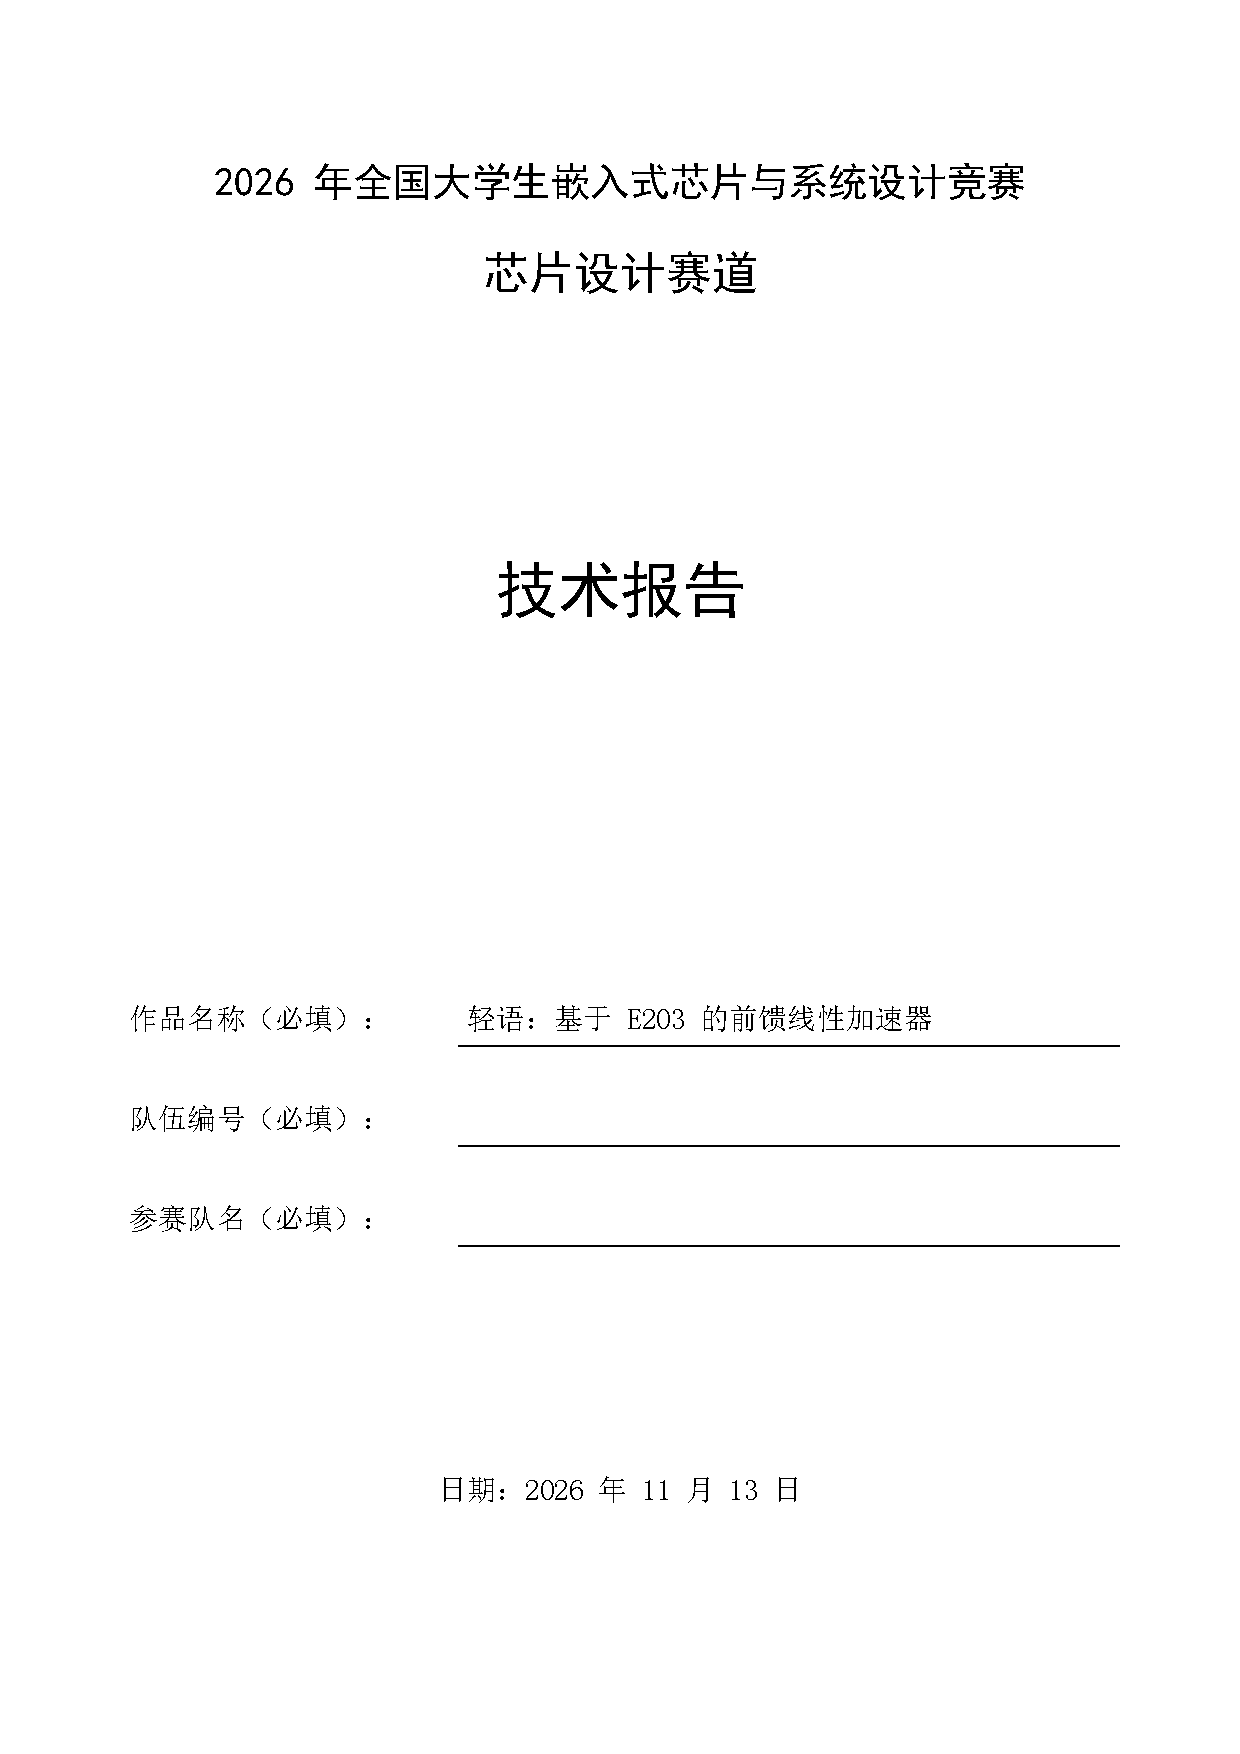
\includepdf[pages=1,pagecommand={\thispagestyle{empty}},fitpaper=true]{assets/cover.pdf}
\pagenumbering{arabic}

\section*{快速预览（一）：做什么，怎样连接}
\addcontentsline{toc}{section}{快速预览}
\begin{center}
{\Large\bfseries 轻语：基于 E203 的前馈线性加速器}\par
\vspace{5pt}
{\small 冻结版本：native12 earlycheck\quad 版本日期：2026 年 11 月 13 日}
\end{center}
本设计面向 KWT-1 语音指令识别模型的前馈网络第一线性层，实现 $99\times64$ 输入与 $64\times256$ 权重的矩阵乘法、偏置处理和定点转换，完整写回 $99\times256$ 个结果。E203 执行控制与驱动，加速器完成数值计算。本报告对应本科必做范围，不包含完整十二层编码器或语音分类硬件实现。

\begin{figure}[H]\centering
\begin{tikzpicture}[node distance=9mm]
\node[box,minimum width=31mm] (cpu) at (0,0) {E203 处理器\\驱动、配置、等待};
\node[box,minimum width=34mm] (load) at (4.2,0) {参数装载主设备\\真实传输与提交};
\node[box,minimum width=37mm] (eng) at (8.7,0) {Q12 加速器 DMA\\读输入、写完整结果};
\node[box,fill=white,minimum width=130mm] (bus) at (4.3,-1.65) {原有 32 位 System Bus 与规定的共享存储访问通路};
\node[box,minimum width=42mm] (ram) at (4.3,-3.2) {512 KiB 共享 SRAM\\保持单一逻辑访问入口};
\draw[arr] (cpu)--(cpu|-bus.north);\draw[arr](load)--(load|-bus.north);\draw[arr](eng)--(eng|-bus.north);
\draw[arr,<->](bus)--(ram);
\node[note,anchor=west,text width=41mm] at (-2,-3.15) {装载、CPU 调度和总线等待均计入任务窗口};
\node[note,anchor=west,text width=41mm] at (7,-3.15) {外部 loader 接口的正式认可仍需闭合};
\end{tikzpicture}
\caption{系统级访问关系。图中三方共用规定通路，不表示三路可独立直连 SRAM。}
\end{figure}

\textbf{三个实现重点。}计算阵列采用 $4\times16$ 个成对乘积单元，复用行、列修正项；片内缓存支持权重装载与计算在合法时隙交叠；输出以固定 signed12 格式保存全部矩阵元素，不再进行 Rice、差分或变长压缩。

\begin{table}[H]\centering\small
\begin{tabularx}{\linewidth}{p{31mm}YY}\toprule
项目 & 本版实现 & 对应依据\\\midrule
数值配置 & X12 / W10 / Y12，最近偶数舍入与饱和 & 源码与软件整数模型\\
计算组织 & 64 个 PE；16 个列 tile；每组最多 4 行 & 冻结 RTL\\
私有存储 & 19.5 KiB 物理容量；使用指定 SRAM 宏 & 宏实例与宽深配置\\
任务完成 & 全部结果写入后，等待最终完成标志的写响应 & SoC 总线检查与物理读回\\
\bottomrule\end{tabularx}
\end{table}
\noindent\textbf{读图约定：}架构图、流程图为依据冻结源码绘制的设计示意；工具截图为实际服务器运行记录，二者不会混称为实物或上板结果。
\clearpage

\section*{快速预览（二）：得到什么，证据到哪里}
\begin{table}[H]\centering
\begin{tabularx}{\linewidth}{p{33mm}p{43mm}Y}\toprule
指标 & 当前结果 & 解释\\\midrule
吞吐量 & \textbf{6075.99 tasks/s} & 150 MHz 换算，历史 12 个完整任务窗口\\
增量面积 & \textbf{0.388582 mm$^2$} & 新增逻辑与私有 SRAM，非整机面积\\
整机平均功耗 & \textbf{约 58.36 mW} & 包含 E203、互连及全部 SRAM\\
单任务能耗 & \textbf{约 9.60 $\mu$J} & 同一网表的 12 窗口工程估计\\
DC setup / hold & $0 / +0.00070456$ ns & 已报告路径非负；完整约束覆盖尚未闭合\\
\bottomrule\end{tabularx}
\end{table}
\begin{figure}[H]\centering
\begin{tikzpicture}
\begin{axis}[width=.88\linewidth,height=46mm,xbar,xmin=0,xmax=.54,bar width=7mm,
 symbolic y coords={当前冻结版本,已核对历史基线,上一版约数},ytick=data,
 xlabel={增量面积（mm$^2$）},nodes near coords,nodes near coords align={horizontal},
 every node near coord/.append style={/pgf/number format/.cd,fixed,precision=4},
 xtick={0,.1,.2,.3,.4,.5},xticklabel style={/pgf/number format/fixed},
 axis lines*=left,enlarge y limits=.3,xmajorgrids=true,grid style={gray!20},
 tick label style={font=\small},label style={font=\small}]
\addplot[fill=accent!70,draw=accent] coordinates {(.388582,当前冻结版本) (.448647,已核对历史基线) (.48,上一版约数)};
\end{axis}\end{tikzpicture}
\caption{面积数值对比。0.48 为上一版实验记录的约数；不同版本并非单因素消融实验。}
\end{figure}
相比上一版约数 6000 tasks/s、0.48 mm$^2$，本版吞吐约提高 1.3\%，面积约降低 19.0\%；相对已核对的 0.448647 mm$^2$ 综合基线，面积降低约 13.4\%。当前能耗数值高于早期记录 7 $\mu$J，且旧值缺少同口径报告，因此不宣称能效改善。

\textbf{已经完成的验证：}12 个本地合成任务及 12 个厂家 SRAM 模型任务逐值核对；每任务检查 25344 个输出值、总线事务守恒和最终物理 SRAM 内容；两种输出身份错误注入验证反压条件下的错误排空。

\textbf{仍需闭合：}正式 600 样本数值精度、loader 平台接口认可、未约束端点的完整时序检查、严格等价审计，以及功耗活动与库外推警告。以上缺项已写入正文；本版冻结不代表这些项目已经合格。

\noindent\textbf{交付定位：}源码提交 \code{8731bf4}；冻结标签 \code{q12-submission-20261113-r1}。本报告按该版本编写，后续修改使用独立分支，不拼接不同配置的最优数据。
\clearpage
\begingroup\small\linespread{1.02}\selectfont\setlength{\parskip}{0pt}
\tableofcontents
\endgroup
\clearpage

\section{摘要}
\subsection{中文摘要}
针对端侧语音识别模型中的前馈线性计算，本设计在指定 E203 SoC 平台上实现一套定点矩阵加速器。计算范围为 $99\times64$ 与 $64\times256$ 矩阵相乘并加偏置，结果为完整 $99\times256$ 矩阵。系统采用 X12/W10/Y12 数值配置，以最近偶数舍入、算术移位和饱和处理完成数值转换。权重和偏置的格式转换采用固定规则，不进行重训、微调或按评测样本拟合参数。

计算阵列由 $4\times16$ 个成对乘积处理单元组成，利用行、列修正项复用减少矩阵计算中的乘法次数。输入、权重与元数据保存在指定 SRAM 宏构成的私有缓存中；装载控制与计算控制分离，权重通过四个槽位循环复用。DMA 保持原有 32 位 System Bus 访问通路，输入参数装载、CPU 调度、总线等待和完整结果写回均纳入任务窗口。输出使用每元素 12 位的固定数值格式，不再对结果进行独立压缩。

冻结版本在历史 12 个任务和厂家 SRAM 模型下通过完整数值及总线检查，平均任务周期为 24687.33，以 150 MHz 换算吞吐为 6075.99 tasks/s。官方 TT、1.10 V、25 $^\circ$C 条件下，增量综合面积为 0.388582 mm$^2$，整机面积为 2.730734 mm$^2$。基于同版网表与 12 个任务活动窗口，整机功耗工程估计为 58.36 mW，平均单任务能耗为 9.60 $\mu$J。已报告 DC 路径的 setup 和 hold slack 分别为 0 和 +0.00070456 ns，但仍存在未约束端点；功耗及严格等价审计也有未闭合项。正式 600 样本精度尚未完成，因此本报告区分已测结果、条件性结论和待验收事项。

\noindent\textbf{关键词：}E203；前馈线性层；定点量化；成对乘积；System Bus；SRAM；综合评估

\subsection{English Abstract}
This work implements a fixed-point feed-forward linear accelerator on the prescribed E203 SoC platform. It computes a $99\times64$ input matrix multiplied by a $64\times256$ weight matrix, adds bias, and stores the complete $99\times256$ output matrix. The X12/W10/Y12 representation uses round-to-nearest-even and saturation. Weight and bias conversion follows fixed rules without retraining, fine-tuning, or fitting to evaluation samples.

The datapath contains a $4\times16$ pair-product array with shared row and column correction terms. Dedicated SRAM macros hold input, weight, and metadata buffers. Separate loading and computation controllers reuse four weight slots. All shared-SRAM traffic follows the original 32-bit System Bus path, and timing includes loading, CPU scheduling, bus stalls, and final writeback. Each output occupies a fixed 12-bit field; no separate output compression is applied.

The frozen design passed twelve historical full-task tests with vendor SRAM models. Its mean latency is 24687.33 cycles, corresponding to 6075.99 tasks/s at 150 MHz. At TT, 1.10 V and 25 $^\circ$C, the incremental mapped area is 0.388582 mm$^2$, while total SoC area is 2.730734 mm$^2$. Twelve activity windows on the same netlist yield an engineering estimate of 58.36 mW and 9.60 $\mu$J per task. Reported setup and hold slacks are 0 and +0.00070456 ns, respectively. Unconstrained endpoints, power-model warnings, strict equivalence review, and the official 600-sample accuracy evaluation remain open; the measurements are not presented as complete signoff.
\clearpage

\section{设计平台与工具}
\subsection{任务范围与系统条件}
赛题采用 KWT-1 开源预训练模型，前馈网络维度为 $64\rightarrow256\rightarrow64$。本设计覆盖本科必做的第一线性层，输入由指定模型的对应层处理流程离线提取；GELU、第二线性层、注意力和完整分类链路均不属于本版已实现范围\cite{guide}。软件数值模型用于生成和核对参考值，不代替加速器必做计算。

平台保留 E203、原总线及外设框架，系统共享 SRAM 为 512 KiB。工作频率目标为 150 MHz；常开域低速时钟按照原平台保留。设计交付覆盖 RTL、功能仿真与逻辑综合，结果来自上述前端设计阶段的测量与检查\cite{hbird,source,eda}。

\begin{table}[H]\centering\small
\caption{工具和资源的职责分工}
\begin{tabularx}{\linewidth}{p{35mm}YY}\toprule
工具或资源 & 用途 & 本报告采用的证据\\\midrule
Verilator / Icarus & 合成数据整机验证与定向检查 & 本地 12 任务结果、错误注入记录\\
Yosys & 选定算术/局部变换的一致性检查 & 局部检查记录；不替代整机 LEC\\
VCS 与厂家 SRAM 模型 & 与宏时序行为相关的整机任务回放 & 12 个完整窗口、物理读回与活动文件\\
Design Compiler & 同版整机综合、面积及约束检查 & 映射网表、SDC、setup/hold 与面积报告\\
Formality & RTL 与映射网表等价检查 & 通过点、未匹配点、黑盒与告警记录\\
PrimeTime 功耗分析 & 读取同版网表与活动估计整机功耗 & 12 窗口功耗、单位与覆盖检查\\
指定标准单元和 SRAM 库 & 综合映射和功耗/时序模型 & TT、1.10 V、25 $^\circ$C；宏实例计数\\
\bottomrule\end{tabularx}
\end{table}

\subsection{测量配置和文件身份}
本版计算引擎文件的 SHA-256 为\par
\noindent\small\path{9447724c51ee9e4e80e72818cf1a448002b485fb00956be98d3f1a9f5848d432}\normalsize\par
同一映射网表 SHA-256 为\par
\noindent\small\path{3eb43b4d79bbeb0389f4bb272e93629e7241dc1a6186c4e6c37a8b7bd448b712}\normalsize\par
吞吐、面积、时序及功耗转录均绑定这一配置。原始网表、约束、活动及工具报告保留在授权服务器的独立运行目录，公开工程提供源码、固件、编译顺序、哈希清单和复现说明。工艺库、厂家模型及私有样本不随公开源码分发。

\subsection{如何理解本报告中的测量}
“历史 12 任务”指已有冻结任务包的厂家模型回放，不等于组委会最终抽取的性能任务；“本地 12 任务”使用合成数据与行为 SRAM，承担功能压力验证，不作为比赛吞吐值。面积是指定库条件下的综合结果，功耗是布局前活动估计，两者均不是芯片实测。对每项指标保留其来源和适用范围，避免把局部测试结论扩展为全部验收通过。
\clearpage

\section{设计原理与系统组成}
\subsection{整体计算与控制流程}
任务由 E203 通过 MMIO 启动。软件先建立任务 epoch 和装载请求，再配置输入基址、输出基址、总字数与已提交边界。装载主设备通过真实总线写入共享 SRAM，只有完成对应写响应后才发布可读边界。加速器仅访问已提交的数据范围；计算过程中软件继续提交后续权重块。最后完整矩阵写回并提交完成标志，E203 检查状态及格式头。

\begin{figure}[H]\centering
\begin{tikzpicture}[node distance=6mm]
\node[box,text width=117mm] (a) {E203 建立 epoch，配置基址与装载请求};
\node[box,text width=117mm,below=of a] (b) {装载数据经原 System Bus 写入共享 SRAM，写响应后发布提交边界};
\node[box,text width=117mm,below=of b] (c) {DMA 读取已提交输入，输入解码与行因子计算，写私有 X 缓存};
\node[box,text width=117mm,below=of c] (d) {权重组装载及列因子计算，与前一组计算按缓存时隙交叠};
\node[box,text width=117mm,below=of d] (e) {$4\times16$ PE 阵列计算，行列修正、偏置、舍入与饱和};
\node[box,text width=117mm,below=of e] (f) {固定 signed12 输出经 DMA 写回，最终标志写响应后完成};
\foreach \u/\v in {a/b,b/c,c/d,d/e,e/f}\draw[arr](\u)--(\v);
\end{tikzpicture}
\caption{一次任务的完整流程。计算和装载存在重叠，图中顺序描述数据依赖，不表示所有阶段完全串行。}
\end{figure}

控制、DMA 和数值计算分别由 \code{qingyu_q12_stream_fio}、\code{q12_icb_stream_prefix} 与 \code{q12_task4} 等模块承担。原 E203 控制端与自有 DMA 入口分离，但计算输入、权重及结果全部经过规定的共享 SRAM 通路。输出矩阵由硬件生成，测试平台只提供输入和执行独立检查。

\subsection{成对乘积与行列修正复用}
对于长度 64 的整数点积，令 $x_k$ 表示输入行、$w_k$ 表示某输出列权重。按相邻元素成对分组，有
\begin{align}
S &= \sum_{k=0}^{31}(x_{2k}+w_{2k+1})(x_{2k+1}+w_{2k}),\\
R &= \sum_{k=0}^{31}x_{2k}x_{2k+1},\qquad
C = \sum_{k=0}^{31}w_{2k}w_{2k+1},\\
\sum_{k=0}^{63}x_kw_k &= S-R-C.
\end{align}
展开每一对的乘积即可得到上述恒等式，因此重排本身不引入近似。对矩阵而言，$R_i$ 在同一输入行的 256 个输出列之间复用，$C_j$ 在同一权重列的 99 个输入行之间复用。偏置在修正之后加入，数值转换在最终结果端进行。

直接矩阵乘法需要 $99\times256\times64=1\,622\,016$ 次标量乘法。按该恒等式计数，主项为 811008 次，行修正 3168 次，列修正 8192 次，合计 822368 次，理论标量乘法次数减少约 49.3\%。这个数字不包含流水寄存器、求和与修正开销，也不能直接换算成 49.3\% 的面积或时延下降。

\begin{figure}[H]\centering
\begin{tikzpicture}
\node[box,text width=28mm] (x) at (0,1) {$x_{2k}+w_{2k+1}$\\13 位有符号};
\node[box,text width=28mm] (y) at (0,-.6) {$x_{2k+1}+w_{2k}$\\13 位有符号};
\node[box,text width=22mm] (m) at (4,.2) {乘法流水\\26 位乘积};
\node[box,text width=26mm] (s) at (7.6,.2) {累加 32 对\\31 位主项};
\node[box,text width=32mm] (q) at (7.6,-1.8) {共享修正与偏置\\32 位中间结果};
\node[box,text width=28mm] (o) at (3.7,-1.8) {RNE 与饱和\\signed12 输出};
\draw[arr](x.east)--(m.north west);\draw[arr](y.east)--(m.south west);\draw[arr](m)--(s);\draw[arr](s)--(q);\draw[arr](q)--(o);
\node[note,text width=36mm] at (0,-1.8) {行因子按行复用\\列因子按列复用};
\end{tikzpicture}
\caption{单个成对乘积通路及共享后处理。W10 数值在本冻结版缓存和 PE 输入处仍符号扩展为 12 位。}
\end{figure}

\subsection{并行阵列与分块调度}
阵列每次处理最多 4 行、16 列，共 64 个输出位置。256 列划分为 16 个 tile，99 行划分为 25 个行组，最后一组仅有 3 行有效。每个点积发出 32 对读请求，控制器根据有效行数屏蔽补齐位置。PE 接收 first/last 标记，first 使用零初值参与第一项累加，last 发布结果有效，避免跨任务残留数据进入有效结果。

\begin{figure}[H]\centering
\begin{tikzpicture}[x=8mm,y=8mm]
\foreach \r in {0,...,3}{\foreach \c in {0,...,15}{\draw[draw=ink,fill=pale](\c,-\r) rectangle +(0.88,-0.82);}}
\foreach \r in {0,...,3}{\node[anchor=east,font=\small]at(-.3,-\r-.4){行 \r};}
\node[note]at(7.5,0.9){每行复用一对 X；每列复用一对 W};
\node[note]at(7.5,-4.4){16 列并行 $\times$ 4 行；最后行组屏蔽第 4 行};
\draw[arr](0,-5.2)--(15.8,-5.2);\node[fill=white,font=\small]at(7.8,-5.2){列 tile：0 到 15，顺序覆盖全部 256 列};
\end{tikzpicture}
\caption{计算阵列组织示意。小方框表示 PE，不是芯片版图。}
\end{figure}

阵列完成一组结果后，将 64 路主项及行因子转入显式结果快照。后处理端每次选择 4 个结果完成行列修正、偏置和量化，阵列可在下游允许时开始下一行组。输出快照保留 tile 和行组身份，后续写回使用相同身份检查，因此性能交叠不会改变矩阵元素的归属。

\subsection{私有 SRAM 与合法时隙复用}
本版通过 16 位宏条带组合形成不同宽度的缓存。X 缓存按四行组织，在一个读请求中送出四对输入；权重缓存同时提供 16 列的权重对。私有权重槽位共四个，以 tile 身份和有效位管理占用状态：只有全部权重及元数据提交后才标记可用，只有对应 tile 的最终结果被接受后才释放。

\begin{table}[H]\centering\small
\caption{冻结版本私有 SRAM 物理组织}
\begin{tabularx}{\linewidth}{p{25mm}p{28mm}p{41mm}Y}\toprule
用途 & 宽度 $\times$ 深度 & 宏组成 & 容量\\\midrule
输入 X & $96\times1024$ & 6 个 RAMSP1024X16 & 12 KiB\\
权重 W & $384\times128$ & 24 个 RAMSP128X16 & 6 KiB\\
行修正项 & $32\times128$ & 2 个 RAMSP128X16 & 0.5 KiB\\
列修正与元数据 & $64\times128$ & 4 个 RAMSP128X16 & 1 KiB\\\midrule
合计 & -- & 30 个 128 深度宏及 6 个 1024 深度宏 & 19.5 KiB\\
\bottomrule\end{tabularx}
\end{table}

权重装载端使用三个有界突发缓冲，每个缓冲聚集 8 个 48 位输入字形成一个 384 位写入字。只有计算侧不发起该缓存读操作的边沿才允许写入；元数据写入同样避开对应读取状态。这里的并行指内部独立存储和调度的交叠，不是增加共享 SRAM 的访问端口。

全 SoC 宏实例为 RAMSP128X16、RAMSP1024X16、RAMSP4096X16 各 30、6、80 个，共 116 个。共享 SRAM 的 64 个 RAMSP4096X16 保持不变，其余原平台存储随整机统计。未采用把私有 W 缓存改为 320 位或进一步合并元数据的实验版本，因此不能把这些实验的预期宏节省计入本版。

\subsection{数值格式、舍入与误差来源}
输入保留原 signed12 编码。对原整数权重 $W_{12}$ 和偏置 $b$，转换定义为
\begin{align}
W_{10}&=\sat_{[-512,511]}\bigl(\RNE(W_{12}/4)\bigr),\\
b'&=\RNE(b/4),\qquad s'=s-1,\\
Y_{12}&=\sat_{[-2048,2047]}\left(\RNE\left(\frac{XW_{10}+b'}{2^{s'}}\right)\right).
\end{align}
该转换的输出物理尺度为原 Y13 尺度的两倍。低位舍入造成的量化误差和饱和截断需在软件模型与 RTL 中保持一致，不能用旧版精度成绩替代本版。权重除以 4 后在缓存中进行符号扩展，不会恢复丢弃的精度。

实现使用算术右移、guard 位、sticky 位和保留最低位判断进位。对半值采用偶数舍入，使正负方向具有一致规则；最终按 signed12 范围饱和。对于移位、饱和边界和符号扩展，验证以独立整数参考为准。成对乘积恒等式没有近似误差，主要数值误差来源是输入/权重量化、偏置转换、输出舍入和饱和。

正式精度应按每一层汇总全部 600 条样本的输出误差 RMS，并除以浮点参考 RMS（分母下限 $10^{-8}$），取 12 层中的最大值；本科门槛为 3\%\cite{guide}。本版尚未完成这一评估，不把“与整数模型逐位一致”表述为“满足浮点精度门槛”。

\subsection{完整输出格式与地址映射}
共享 SRAM 必须保存完整矩阵，而不是待软件解压的结果\cite{qa}。本版以固定 signed12 字段顺序保存每个元素，每 8 个元素恰好对应 3 个 32 位字；存储长度不依赖数值大小和零值比例。每个 tile 含 $99\times16=1584$ 个元素，即 19008 位、594 个 32 位字。

\begin{figure}[H]\centering
\begin{tikzpicture}[x=1cm]
\node[box,text width=25mm] (flag) at (0,0) {字 0\\完成标志};
\node[box,text width=32mm] (head) at (3.6,0) {字 1--16\\各 tile 固定长度};
\node[box,text width=46mm] (data) at (8.4,0) {字 17--9520\\16 个完整 tile};
\draw[arr](flag)--(head);\draw[arr](head)--(data);
\foreach \k in {0,...,7}{\draw[fill=pale,draw=ink](\k*1.48-1.3,-1.5) rectangle +(1.48,-.7);\node[font=\small]at(\k*1.48-.56,-1.85){$y_{\k}$};}
\node[note]at(4,-2.6){每个字段恒为 12 位；连续 96 位对应三个 32 位总线字};
\end{tikzpicture}
\caption{完整 signed12 输出布局，不采用结果熵编码或稀疏省略。}
\end{figure}

矩阵共 25344 个数，占 38016 字节；加上 17 字头部，分配空间为 38084 字节（9521 字）。任务开始时先使完成标志失效，结束时再次写入 \code{0x32443151}，因此任务实际写命令为 9522 次。16 个长度字段均为 19008，其单位是位，不是元素数。

设输出列 $j$ 的 tile 为 $t=\lfloor j/16\rfloor$，tile 内列 $c=j\bmod16$，第 $i$ 行对应位偏移为 $b=12(16i+c)$。以 32 位字为单位，目标字偏移为
\[
 a=17+594t+\lfloor b/32\rfloor,\qquad r=b\bmod32.
\]
读取该字及必要的下一字，右移 $r$ 后取低 12 位并符号扩展，即可直接得到 $Y_{i,j}$。固定下标读取不需要压缩解码器。输出写回采用完整长度检查及最终响应确认，不能在最后一个写请求发出时提前结束计时。

\subsection{ICB 传输、反压和错误排空}
DMA 使用 4 项在途请求记录、16 字读缓冲和 8 字写缓冲。每笔命令记录读写归属和结束标记，响应必须按对应归属消费。若总线没有接受已提出的命令，地址、读写方向和载荷保存在保持寄存器中，直到握手完成。新请求选择采用已就绪输出写优先，降低结果反压；该策略只作用于自有 DMA，不改变下游官方总线位宽和协议。

输出身份检查同时核对 tile、字索引与范围。原实现把身份检查使能与 formatter ready 相连，错误排空又影响 ready，形成组合反馈。本版改为只要输出有效即检查身份，再独立产生错误控制，正常任务的有效握手和周期不变。

\begin{figure}[H]\centering
\begin{tikzpicture}
\node[box,text width=31mm] (v) at (0,0) {输出有效及身份\\tile / index};
\node[box,text width=33mm] (check) at (4.4,0) {身份合法性检查\\不依赖下游 ready};
\node[box,text width=30mm] (abort) at (8.7,0) {错误标记与排空\\停止新命令};
\draw[arr](v)--(check);\draw[arr](check)--(abort);
\node[box,text width=33mm] (ready) at (4.4,-1.8) {正常握手控制\\valid 与 ready};
\draw[arr](v.south)|-(ready.west);\draw[arr](abort.south)|-(ready.east);
\end{tikzpicture}
\caption{本版错误检查依赖关系。检查逻辑不再从 ready 取得使能，切断原反馈环。}
\end{figure}

发生错误后系统停止产生新命令，继续接收已发出的响应并排空在途记录；失败任务不能发布有效完成矩阵。分别在 ready 为 1 和 0 时注入非法输出索引的整机测试均通过，观测到 5 周期排空，已发命令数与响应数分别保持 2046/2046 和 2047/2047。

\subsection{固件寄存器与同步协议}
软件配置接口位于 \code{0xf0000000}，装载邮箱位于 \code{0xf0020000}。输出区域从 \code{0xa0000000} 开始，输入区从 \code{0xa0040000} 开始，控制记录位于 \code{0xa0030100}。驱动以 \code{fence rw,rw} 保证提交记录与后续访问的顺序，epoch 避免旧任务就绪记录被新任务误用。

\begin{table}[H]\centering\small
\caption{加速器关键控制寄存器（相对配置基址）}
\begin{tabularx}{\linewidth}{p{19mm}p{31mm}Y}\toprule
偏移 & 用途 & 行为说明\\\midrule
0x00 & 标识 & 读回 \code{0x51313231}\\
0x04 & 启动/清状态 & 空闲时接受启动，拒绝忙态非法重配\\
0x08 / 0x0c & 输入/输出基址 & 启动前配置，4 字节对齐\\
0x10 / 0x14 & 状态/阻塞等待 & 状态含忙、完成、错误；WAIT 等待完成或错误\\
0x18 & 任务计数 & 加速器内部周期诊断，不替代系统完整窗口\\
0x34 / 0x38 & 总输入字数/epoch & 限定数据范围及任务身份\\
0x3c / 0x40 & 可读边界/提交 epoch & 只扩展已实际提交的数据边界\\
\bottomrule\end{tabularx}
\end{table}

CPU 通过阻塞 WAIT 减少重复轮询，但仍检查实际共享控制记录和最终输出头。驱动采样的周期与测试平台完整窗口具有不同边界，本报告吞吐采用后者，而不选取较短的内部核心周期。

\section{验证过程与数据分析}
\subsection{验证层次和通过条件}
验证按数值单元、格式与协议、完整 SoC、厂家模型、综合网表五个层次组织。软件整数点积与 RTL 中的成对乘积实现相互独立，输出读取按固定下标解释共享 SRAM 内容。正常任务之外，保留复位、边界、反压、非法结束和错误排空检查，不能仅凭完成标志判断数值正确。

\begin{figure}[H]\centering
\begin{tikzpicture}[node distance=5mm]
\node[box,text width=121mm] (n) {数值参考：直接整数点积、偏置、RNE、饱和};
\node[box,text width=121mm,below=of n] (p) {模块验证：输出格式、输入解码、握手与反压、复位};
\node[box,text width=121mm,below=of p] (s) {本地整机：12 个合成任务、逐值比较、真实总线守恒};
\node[box,text width=121mm,below=of s] (v) {厂家模型：12 个历史任务、物理 SRAM 读回、完整活动窗口};
\node[box,text width=121mm,below=of v] (g) {综合及映射后：面积、setup/hold、Formality、功耗与覆盖审计};
\foreach\u/\v in {n/p,p/s,s/v,v/g}\draw[arr](\u)--(\v);
\end{tikzpicture}
\caption{验证证据链。各层结论有各自范围，下层通过不自动代表正式验收通过。}
\end{figure}

本地 12 个合成任务的均值为 25647.75 周期，厂家历史 12 任务均值为 24687.33 周期。输入分布不同会改变输入编码长度及总线流量，因此这两个均值不能用来说明“仿真器更快”或设计跨平台性能提升。两组都比较全部输出值，各自覆盖 $12\times25344=304128$ 个数值。

\begin{table}[H]\centering\small
\caption{本版功能与综合检查状态}
\begin{tabularx}{\linewidth}{p{36mm}p{26mm}Y}\toprule
检查项 & 结果 & 解释\\\midrule
本地整机 12 任务 & 通过 & 行为 SRAM、合成数据，输出及总线检查\\
厂家模型 12 任务 & 通过 & 完整写回及物理读回，正常周期与父版逐项相同\\
错误身份注入 & 2/2 通过 & ready=1/0 均排空，不发布完成矩阵\\
Formality 工具比较 & 35565 通过，0 失败 & 仍有未匹配、unread 与解释告警，严格审计未通过\\
正式 600 样本精度 & 未完成 & 不以历史整数检查替代\\
\bottomrule\end{tabularx}
\end{table}

\subsection{计时窗口与吞吐量}
赛题要求从输入和参数开始装载计时，到结果全部写回结束，包含装载、总线等待与 E203 调度\cite{guide,qa}。本版测试保留真实加载请求、共享存储写入、DMA 读回和结果写入的事务计数。任务间复位不计入运行时间，计算机端文件读取及一次性格式转换不计入硬件窗口。

令第 $i$ 个任务耗费 $N_i$ 个系统时钟周期，时钟频率为 $f$，则
\[
T_{\mathrm{task}}=\frac{\sum_i N_i}{Mf},\qquad
\mathrm{Throughput}=\frac{Mf}{\sum_iN_i}=\frac{f}{\overline N}.
\]
取 $M=12$、$f=150\times10^6$ Hz 和 $\overline N=24687.3333$，得到 6075.99 tasks/s。最慢任务为 24802 周期，最快为 24533 周期。该换算以 150 MHz 为条件，完整时序约束尚未闭合的事实在时序小节单独说明。

\begin{figure}[H]\centering
\begin{tikzpicture}
\begin{axis}[width=.94\linewidth,height=57mm,xmin=-.4,xmax=11.4,ymin=24350,ymax=25100,
 xtick={0,1,...,11},xlabel={历史任务编号},ylabel={完整任务周期},
 ymajorgrids=true,grid style={gray!20},scaled y ticks=false,
 ytick={24400,24600,24800,25000},yticklabel style={/pgf/number format/.cd,fixed,precision=0},
 tick label style={font=\small},label style={font=\small},legend style={font=\small,at={(.5,1.03)},anchor=south,legend columns=2}]
\addplot[accent,thick,mark=*] coordinates{(0,24560)(1,24708)(2,24725)(3,24689)(4,24686)(5,24533)(6,24710)(7,24646)(8,24802)(9,24652)(10,24778)(11,24759)};
\addlegendentry{厂家模型完整窗口}
\addplot[warm,dashed,domain=0:11]{25000};\addlegendentry{6000 tasks/s 对应周期}
\end{axis}\end{tikzpicture}
\caption{12 个历史任务的完整周期。纵轴范围为 24350--25100，用于显示任务间差异；不是零基柱状图。}
\end{figure}

\subsection{面积统计与结构影响}
赛题的加速器面积包括新增计算逻辑、接口和内部 SRAM；复用 E203、512 KiB 共享 SRAM、固定总线及外设面积单列\cite{guide}。本版按相同网表进行分项统计，不把整机面积误作增量面积，也不将宏遗漏或重复计入。

\begin{table}[H]\centering
\caption{同版综合面积明细}
\begin{tabularx}{\linewidth}{Yrr}\toprule
项目 & 面积（$\mu$m$^2$） & 面积（mm$^2$）\\\midrule
加速器及私有存储 & 384884.747634 & 0.384885\\
NP3 仲裁逻辑 & 1113.050400 & 0.001113\\
共享路径新增非宏逻辑 & 2584.562400 & 0.002585\\\midrule
增量合计 & 388582.360434 & 0.388582\\
全 SoC 合计 & 2730733.915310 & 2.730734\\
\bottomrule\end{tabularx}
\end{table}

增量结果低于 2.25 mm$^2$ 的逻辑综合预算，但这不是“芯片物理边长已经通过”的证明。成对乘积复用、共享修正、数据寄存器有效位管理及完整输出格式共同作用于面积；本轮没有单独隔离每一项改动的面积收益，不能给出未经测量的逐项百分比。

\subsection{150 MHz 约束与时序修复}
目标周期为 6.666666667 ns，setup 不确定度为 0.1 ns、hold 不确定度为 0.02 ns；数据 I/O 延迟未放宽。loader 导出时钟用 1:1 generated clock 表达，移除误加在该时钟输出上的数据输出延迟。四个 PWM 异步同步器第 0 级入口按异步来源单独约束，后续同步级继续计时，未对加速器、SRAM 或总线数据通路设置泛化 false path。

早期中间版存在 $-0.14896035$ ns 的 SRAM 数据 hold 违例。切断 ready/abort 反馈后完成同版重新综合及 hold-only 修复，最差已报告 setup 为 0 ns、hold 为 +0.00070456 ns。保持裕量约 0.70 ps，余量很小，不能忽略条件变化。

\begin{table}[H]\centering\small
\caption{时序结果与覆盖限制}
\begin{tabularx}{\linewidth}{p{37mm}p{35mm}Y}\toprule
项目 & 当前观测 & 解释\\\midrule
已报告 setup & 0.00000000 ns & 边界达到，不表示存在充足裕量\\
已报告 hold & +0.00070456 ns & SRAM 真实数据路径修复后非负\\
组合环检查 & 原反馈环告警消除 & 错误检查不再依赖 ready\\
未约束端点 & UART、AON 等仍列出 & 3 路 UART 的 24 个锁存器 D 端、2 个 AON 异步入口及 loader 时钟输出需要分类闭合\\
完整时序验收 & 尚未完成 & 不凭非负最差路径宣布全 SoC 通过\\
\bottomrule\end{tabularx}
\end{table}

继承外设锁存器与异步输入需要分别解释其功能、模式和时钟关系。本报告保留这些告警，不通过删除检查或把所有端点设为 false path 来消除报告条目。

\subsection{功耗与能耗的计算口径}
功耗使用同版综合网表和同一任务窗口的 cell-aware SAIF，统计 E203、加速器、互连及全部 SRAM 的动态和静态功耗，不包含模拟模块或片外设备。116 个宏实例逐一匹配，未将缺少模型或活动的 SRAM 当作零功耗。

令窗口长度为 $\Delta t_i$，该窗口整机平均功耗为 $P_i$，则
\[
\overline P=\frac{\sum_iP_i\Delta t_i}{\sum_i\Delta t_i},\qquad
\overline E=\frac{\sum_iP_i\Delta t_i}{M}.
\]
12 个窗口得到时长加权平均功耗 58.3583 mW、平均能耗 9.60339 $\mu$J。原功耗报告 Total Power 只有约四位有效数字，最终结果采用 58.36 mW 与 9.60 $\mu$J，不把转录计算的小数位误当作测量精度。窗口 ps 时长与理想整数周期换算存在时钟仿真精度引起的微小差别，能耗使用实际记录时长。

\begin{table}[H]\centering\small
\caption{12 个历史完整任务及对应功耗窗口}
\begin{tabular}{rrrrr}\toprule
任务 & 周期 & 窗口（$\mu$s） & 功耗（mW） & 能耗（$\mu$J）\\\midrule
00 & 24560 & 163.710294 & 58.50 & 9.577052 \\
01 & 24708 & 164.696862 & 58.40 & 9.618297 \\
02 & 24725 & 164.810184 & 58.40 & 9.624915 \\
03 & 24689 & 164.570208 & 58.40 & 9.610900 \\
04 & 24686 & 164.550210 & 58.30 & 9.593277 \\
05 & 24533 & 163.530312 & 58.30 & 9.533817 \\
06 & 24710 & 164.710194 & 58.30 & 9.602604 \\
07 & 24646 & 164.283570 & 58.20 & 9.561304 \\
08 & 24802 & 165.323466 & 58.40 & 9.654890 \\
09 & 24652 & 164.323566 & 58.40 & 9.596496 \\
10 & 24778 & 165.163482 & 58.30 & 9.629031 \\
11 & 24759 & 165.036828 & 58.40 & 9.638151 \\
\bottomrule\end{tabular}

\end{table}

功耗流程完成不等于严格验收通过。首窗口 \code{check_power} 报告 215 个 slew 超表、2685 个负载超表及 3 个无逻辑函数库单元；活动来源属性在所用工具版本下存在兼容问题，完整覆盖与外推警告尚未闭合。因此这些数字标为工程估计，不是无警告签核值。

\subsection{综合前后等价性及其边界}
同一 RTL、mapped.v 和 mapped.svf 的 Formality 工具结果显示 Verification SUCCEEDED，35565 个比较点通过、0 个失败点。然而仍有 625 个 unread 点、9 个仅参考侧未匹配寄存器及 RTL 解释告警。9 个未匹配点分布在原总线合并控制、AON PMU 计数器与输入解码器状态中，尚未逐项完成独立判定。

SRAM 采用两侧对应的对称黑盒，黑盒匹配完成；没有 dont\_verify 点和用户定义常量。该证明范围止于 SRAM 边界，并不证明宏内部实现。严格审计保留未匹配点等条件，当前不能用工具成功字符串代替完整等价验收。

\section{分析与讨论}
\subsection{版本对比及解释限制}
\begin{table}[H]\centering\small
\caption{历史数值与本版结果对比}
\begin{tabularx}{\linewidth}{Yrrr}\toprule
版本或记录 & 吞吐（tasks/s） & 面积（mm$^2$） & 能耗（$\mu$J）\\\midrule
本版冻结配置 & 6075.99 & 0.388582 & 9.60$^{*}$\\
已核对历史面积基线 & -- & 0.448647 & --\\
上一版记录（约数） & 6000 & 0.48 & --\\
早期版本记录 & 4700 & 0.38 & 7\\
\bottomrule\end{tabularx}
\captionnote{$^{*}$本版能耗为整机工程估计。其余历史记录缺少同网表、同窗口、同角及活动覆盖报告；空白项表示未提供，不代表零。}
\end{table}

本版面积相对已核对基线减小约 13.4\%，相对上一版约数减小约 19.0\%；吞吐略高于 6000 tasks/s。当前能耗估计高于早期记录，但旧版本缺少可复核的同口径报告，不能将两者之差直接归因于某项 RTL 改动。不同版本的输出格式、任务窗口、数值精度与验收条件需要一并比较。

面积节省与能耗改善不是同一件事。更小的逻辑可能伴随更长的运行时间、更频繁的存储访问，整机静态和 CPU 开销也持续累积。本版完整输出增加确定性的总线写入量，相比旧压缩输出版本不能仅比较计算阵列的动态功耗。后续优化应观察总任务能量，而不只观察瞬时功率。

\subsection{吞吐瓶颈与优化顺序}
在 150 MHz 下达到 6000 tasks/s 的平均周期预算为 25000，本版均值距离预算只余约 313 周期。达到 10450 tasks/s 则平均周期需降至约 14354，要求比当前减少约 41.9\%。计算阵列按 25 个行组、16 个列 tile、每点积 32 对计算，仅主计算读请求就有 12800 个发出周期；这不是端到端下界证明，但说明可用于装载、状态切换和完整写回的余量会非常紧张。

输出本身固定需要 9522 个写命令。共享 SRAM 保持单一 32 位访问入口，因此增加更多 PE 并不保证端到端吞吐同比增加。更合理的次序是先量化总线空泡、已提交数据等待和输出反压，再判断计算阵列是否成为主要瓶颈。本轮没有给出各类等待的独立百分比分解，不绘制未经测量的周期占比图。

可以继续研究的方向包括：在原协议能力内提高请求连续性；缩短提交和状态切换空泡；在完整输出不变的前提下压缩私有缓存冗余位；减少不必要的数据翻转。每一方向都必须重跑同版功能、150 MHz 时序、面积和能耗检查。共享 SRAM 直连、扩大接口位宽或省略输出值不属于可采用的优化路径。

\subsection{规则核对与当前完成情况}
\begin{longtable}{p{26mm}p{82mm}p{37mm}}
\caption{与赛题要求对应的实现和边界}\label{tab:rules}\\
\toprule 项目 & 本版处理 & 状态\\\midrule\endfirsthead
\toprule 项目 & 本版处理 & 状态\\\midrule\endhead
第一线性层 & 完成矩阵乘法、偏置、量化及完整输出，CPU/TB 不代算 & 整数功能通过\\
多层参数切换 & 历史包覆盖 12 个对应任务，每任务真实装载 & 历史验证通过\\
不重训规则 & 固定离线 RNE 变换、重排与输入打包 & 有转换脚本；正式精度待测\\
完整输出 & 25344 个固定 signed12 字段，无另行压缩 & 已实现及物理读回\\
规定通路 & 保持 32 位 System Bus 与共享 SRAM 逻辑入口 & 无旁路；loader 认可待闭合\\
完整计时 & 输入/权重装载、等待、调度及最终写响应计入 & 历史窗口已记录\\
150 MHz & 已报告 setup/hold 非负，仍有未约束端点 & 全约束验收未完成\\
面积上限 & 增量 0.388582 mm$^2$，上限 2.25 mm$^2$ & 该配置综合数值满足\\
整机功耗 & 含 CPU、互连和所有 SRAM，12 窗口同网表 & 估计完成，严格审计未闭合\\
数值门槛 & 600 样本、逐层 NRMSE 最大值不超过 3\% & 未完成\\
同版一致性 & 配置、源文件和网表哈希绑定 & 已建立，不混用最优值\\
\bottomrule
\end{longtable}

\subsection{工程经验与后续工作}
本轮最直接的经验是先固定访问通路、任务边界和数据格式，再讨论性能数字。输出是否完整、装载是否实际发生、最后写响应是否计入，都会改变吞吐和能耗的含义。以哈希绑定源文件、网表和活动窗口，使每个结果能回到同一份设计，避免“最快仿真”和“最小综合面积”来自不同配置。

当前代码作为保底提交基线冻结，后续修改保存在独立分支。优先工作依次是：补齐正式数值精度入口；解释并闭合外设未约束端点；逐项处理等价未匹配/解释告警；核查功耗活动来源和模型超表；最后再按可复核周期分解进行性能优化。每次确认改进后更新独立版本的证据，不覆盖本报告的原始记录。

\section{原始记录与复现入口}
\subsection{源码、模型与报告的对应关系}
公开仓库冻结提交为 \code{8731bf4}，完整提交标识如下：
\begin{center}\small\code{8731bf4f553e80a1ac5e68fb924b0436ddbdb77f}\end{center}
交付入口 \path{final/q12_submission_20261113/} 包含完整源文件树、固件、编译顺序、验证脚本和冻结清单。文件 \code{FREEZE_MANIFEST.json} 对 169 个源及证据文件记录哈希，交付清单进一步绑定报告和原始图片。

本报告的数字来自 \code{earlycheck_observation.json}、\code{power_observation.json} 及服务器原始工具显示，图表的计算只进行单位换算和明确公式求值。附图保留有利和不利结果。历史时间点截图中的“运行中”或首轮失败记录不代表最终状态，最终判断以本报告相应小节说明为准。

\begin{table}[H]\centering\small
\caption{复现与核验入口}
\begin{tabularx}{\linewidth}{p{48mm}Y}\toprule
入口 & 作用与依赖\\\midrule
\code{final/.../verify.py} & 检查冻结文件 SHA-256，不启动 EDA，也不代表验收通过\\
\code{run_local.py} & 以 \code{--storage-bits 12 --weight-bits 10 --write-priority --early-output-check} 生成同候选的合成任务验证\\
\code{check_output_fault.py} & 在已构建的本地整机环境中验证两类错误排空\\
\code{run_earlycheck_full.py} & 历史服务器整机综合、厂家模型回放及 Formality 流程；带本轮时间边界\\
\code{run_power_recovery.py} & 同版功耗重放及所用工具版本兼容处理\\
\bottomrule\end{tabularx}
\end{table}
表中实验脚本位于 \path{experiments/q12_dense_20261113/} 及其 \path{server/} 子目录。服务器脚本依赖已恢复的授权原始包、工艺库、模型与私有任务，并包含历史运行目录/时限；新环境需按 README 恢复依赖，不能把它们原样运行视为一键完成正式评测。

\subsection{原始图片说明}
后续五页给出实际服务器截图，分别用于检查测量汇总、未约束端点、SRAM hold 路径、功耗覆盖与警告、等价结果与未匹配点。为保留终端内容和小字可读性，证据页采用横向 A4；图片按比例放置，不裁掉失败、警告或边界内容。它们是 EDA 记录，不是实物照片。

\begin{landscape}
\begin{figure}[p]\centering
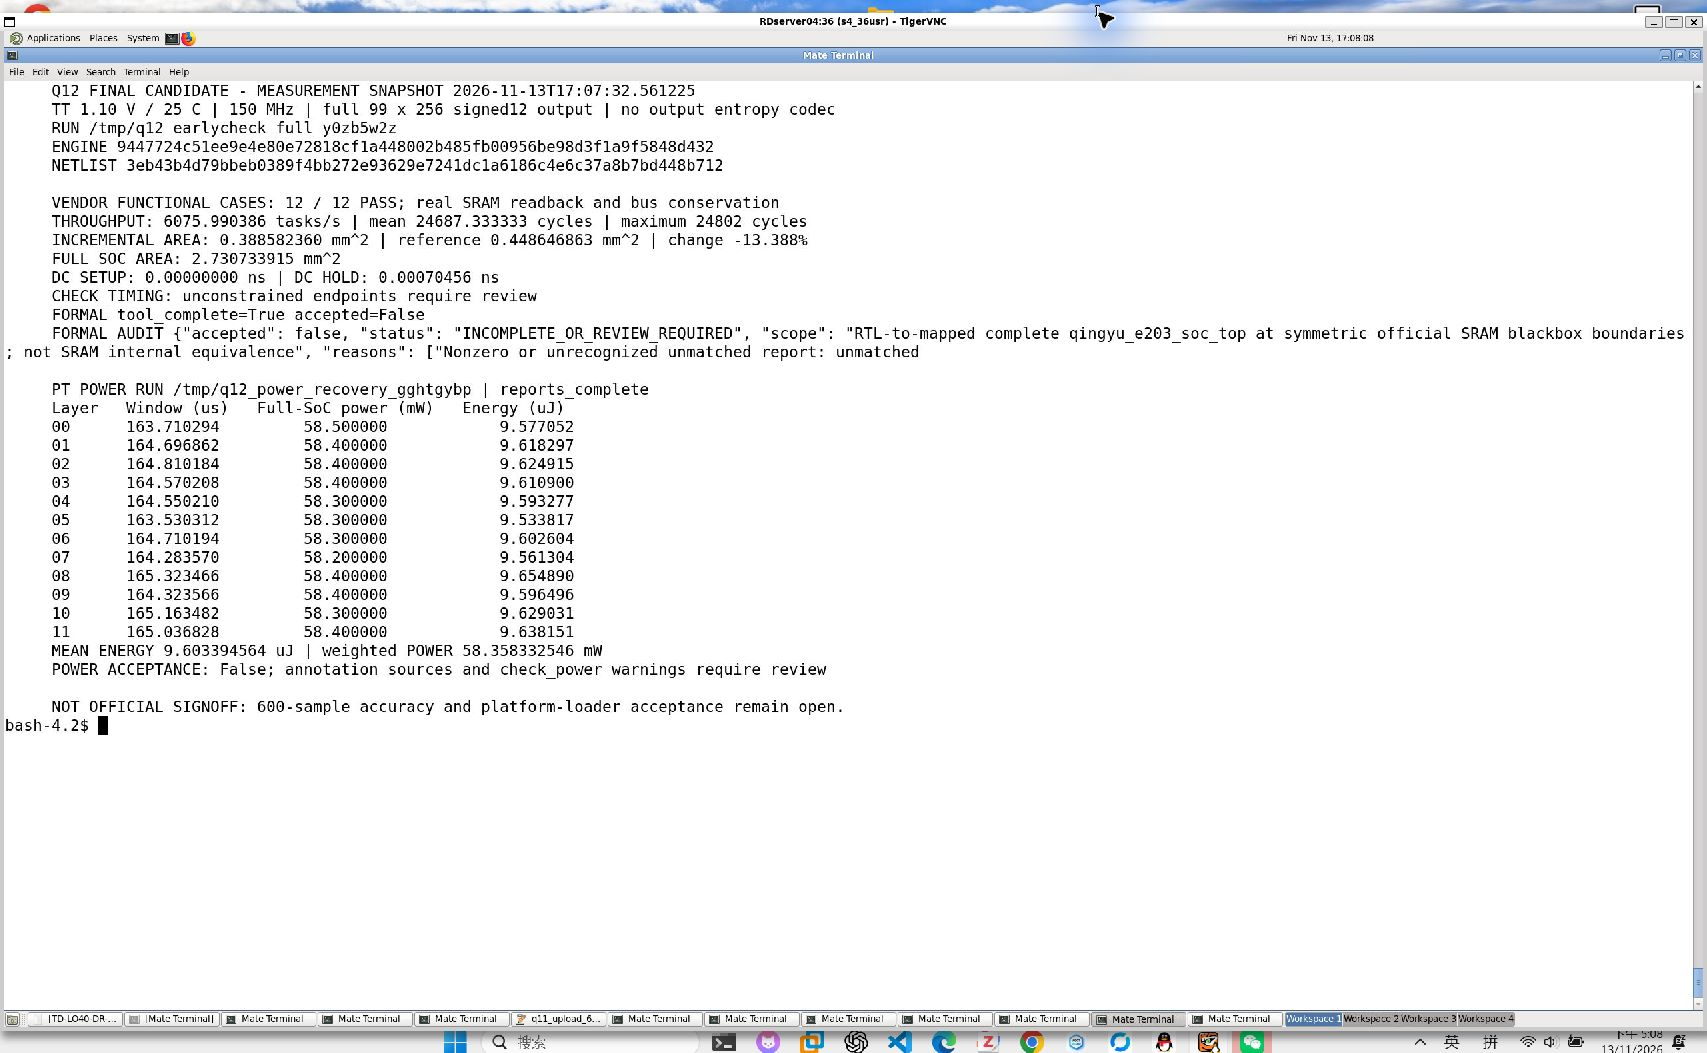
\includegraphics[width=.98\linewidth,height=.80\textheight,keepaspectratio]{assets/26_measurement_comparison.png}
\caption{原始记录 A：同一冻结网表的吞吐、面积与 12 窗口功耗汇总。图中同时保留“非最终签核”的标记。}
\end{figure}\clearpage
\begin{figure}[p]\centering
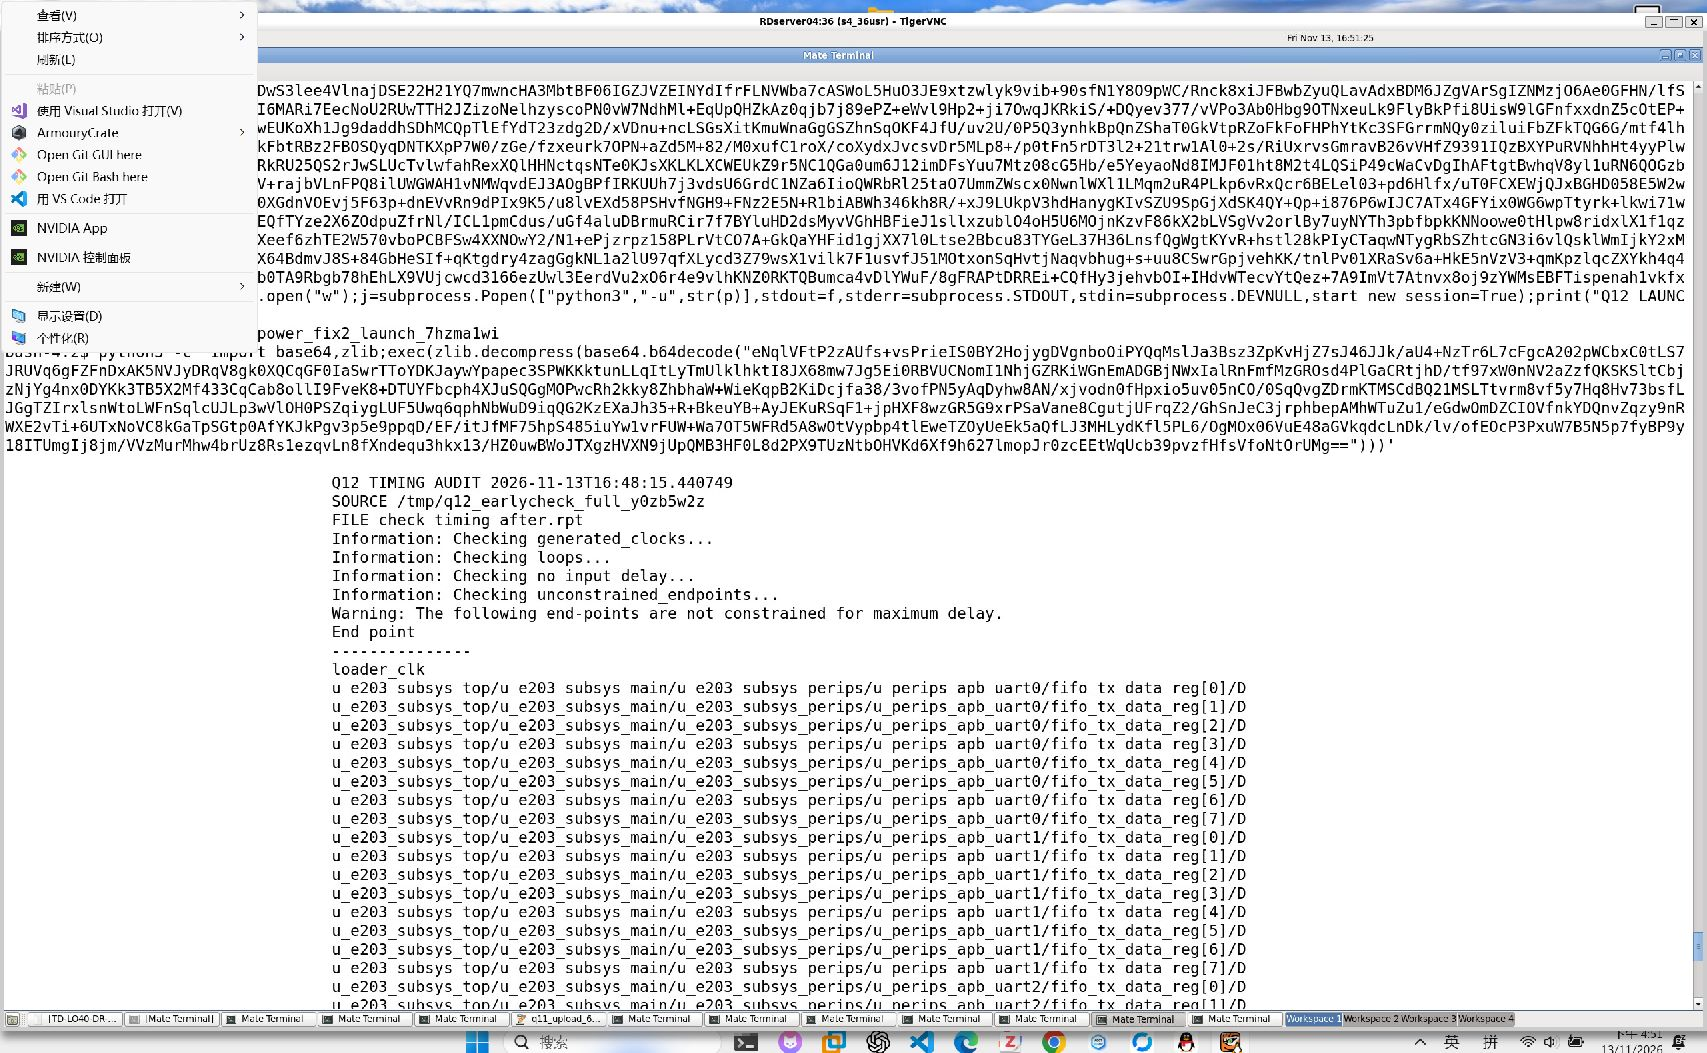
\includegraphics[width=.98\linewidth,height=.80\textheight,keepaspectratio]{assets/24_timing_check_header.png}
\caption{原始记录 B：check\_timing 列出的未约束端点。不能仅凭 setup/hold 非负宣称全部时序合格。}
\end{figure}\clearpage
\begin{figure}[p]\centering
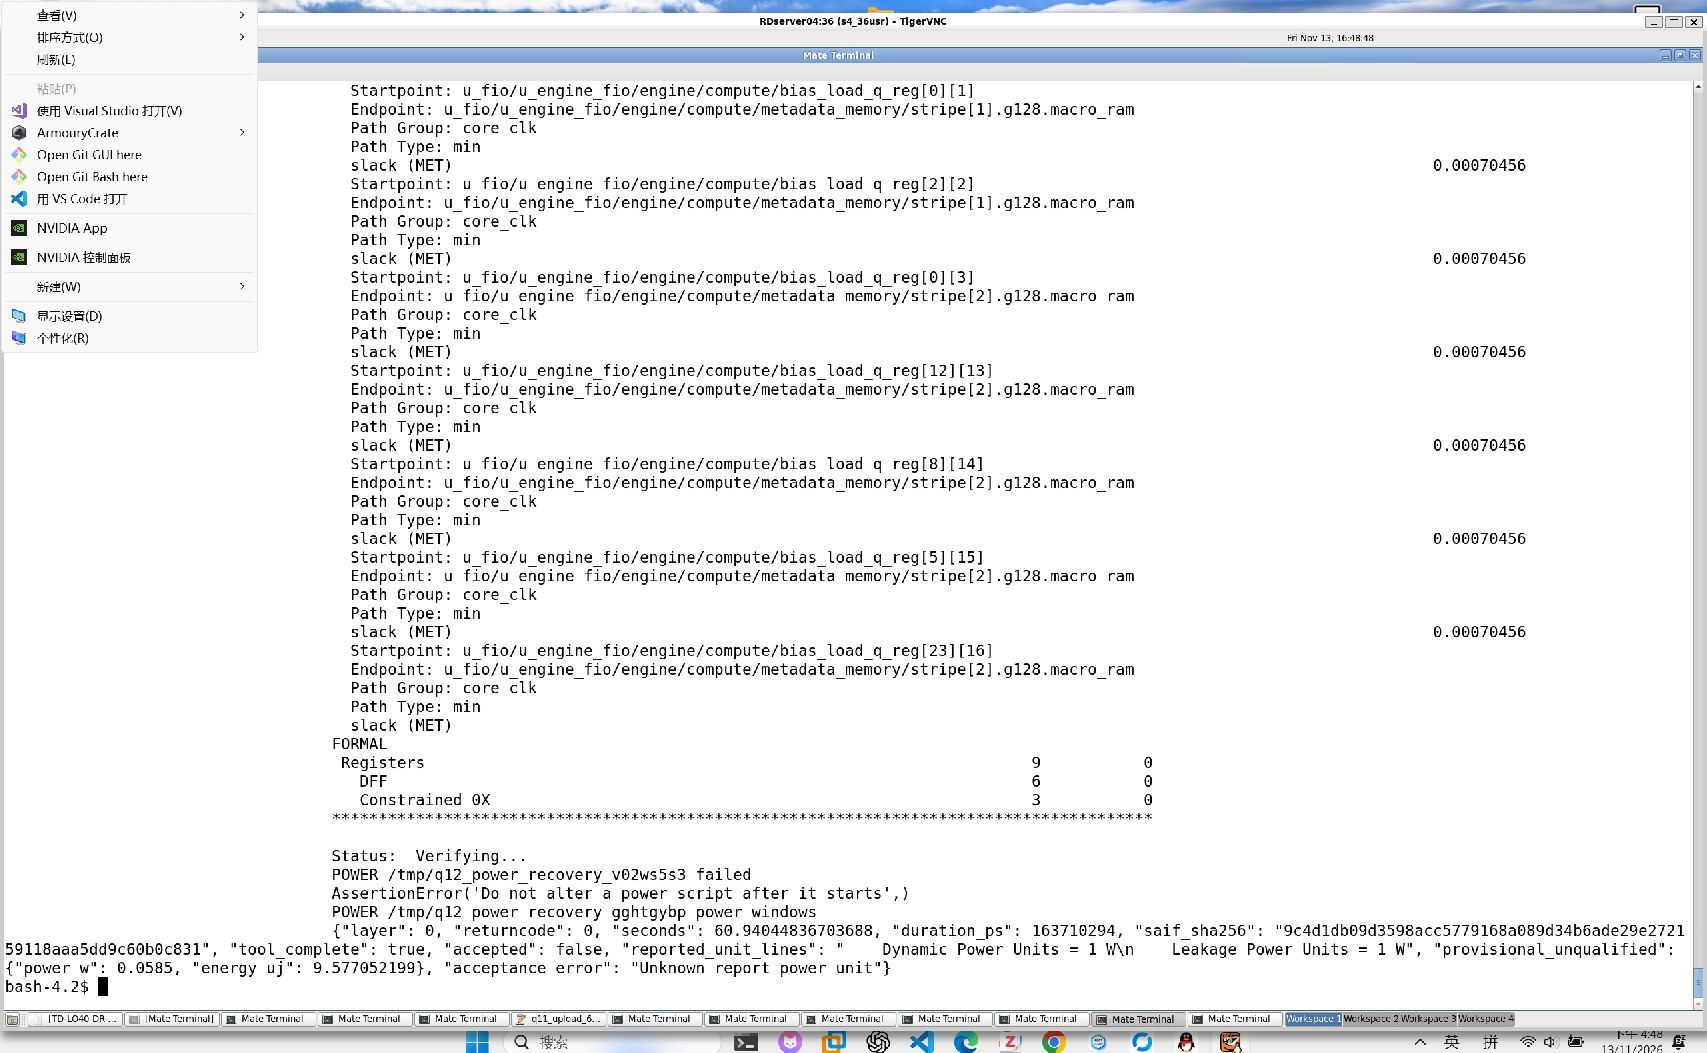
\includegraphics[width=.98\linewidth,height=.80\textheight,keepaspectratio]{assets/22_timing_audit_tail.png}
\caption{原始记录 C：SRAM 数据路径 hold slack 为正。截图中的首轮功耗恢复失败为历史过程，后续重放结果见数据表。}
\end{figure}\clearpage
\begin{figure}[p]\centering
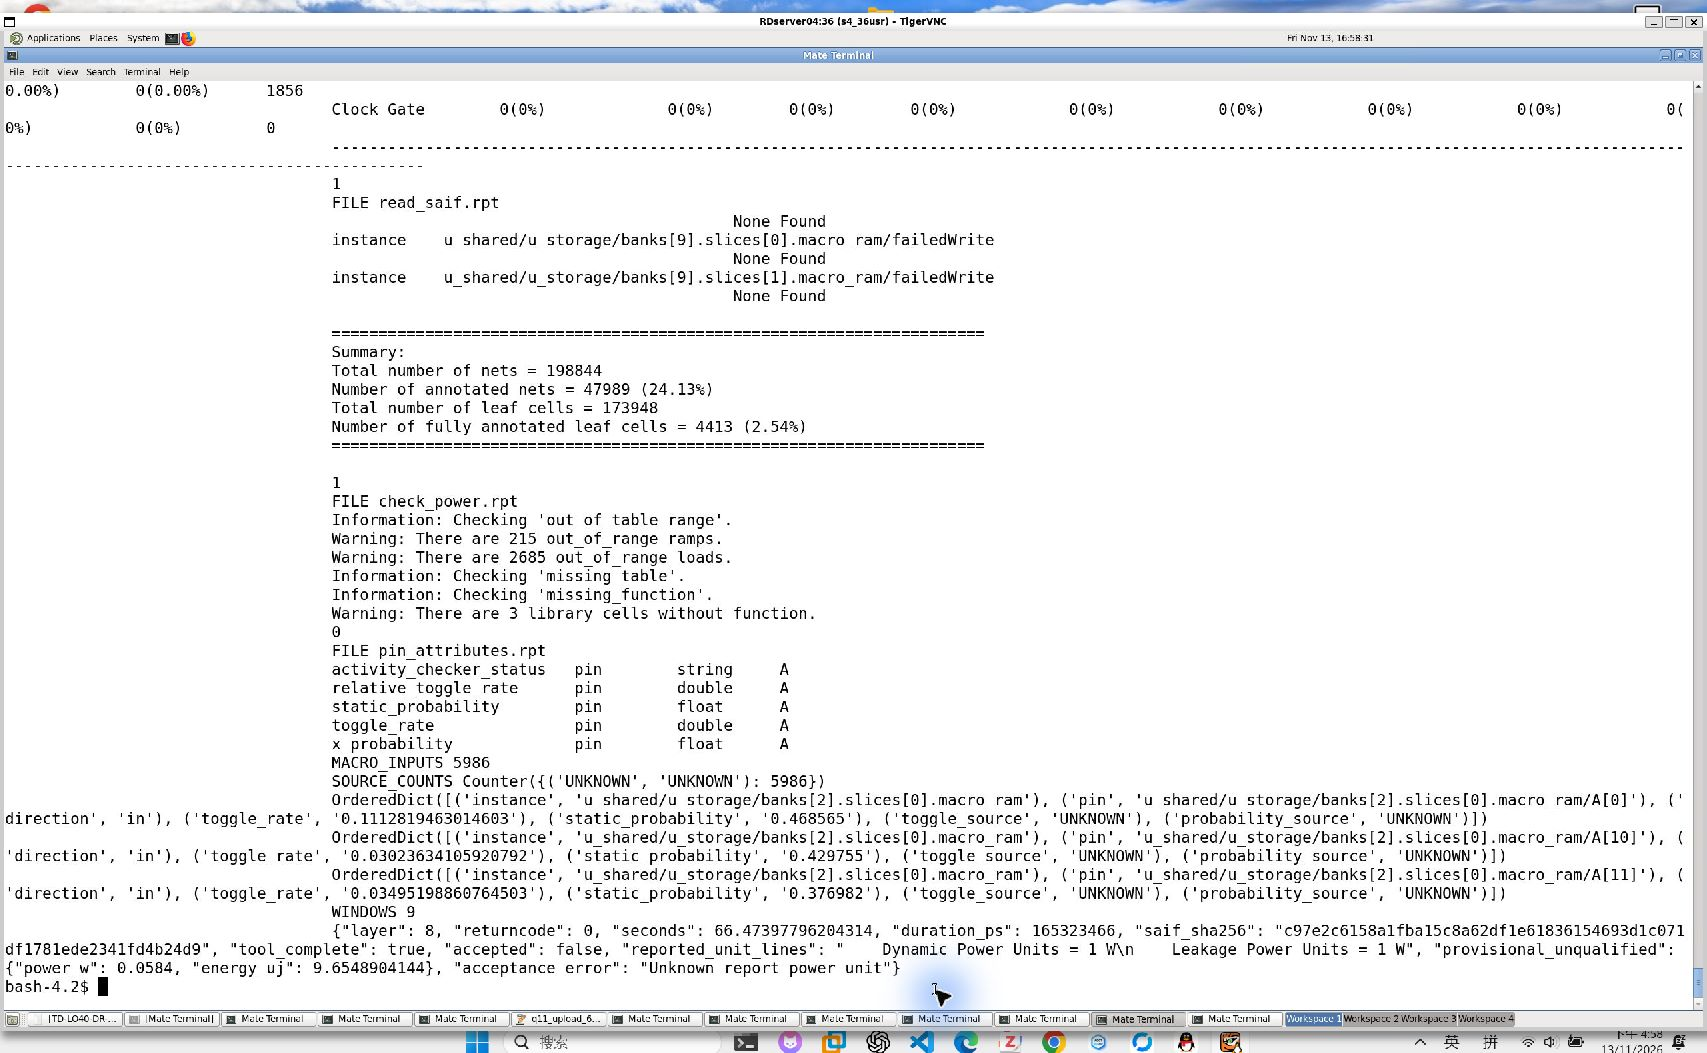
\includegraphics[width=.98\linewidth,height=.80\textheight,keepaspectratio]{assets/25_power_activity_sources.png}
\caption{原始记录 D：活动注入、宏引脚属性及 check\_power 警告。覆盖率需结合传播结果审核，不能把未注入部分当作零活动。}
\end{figure}\clearpage
\begin{figure}[p]\centering
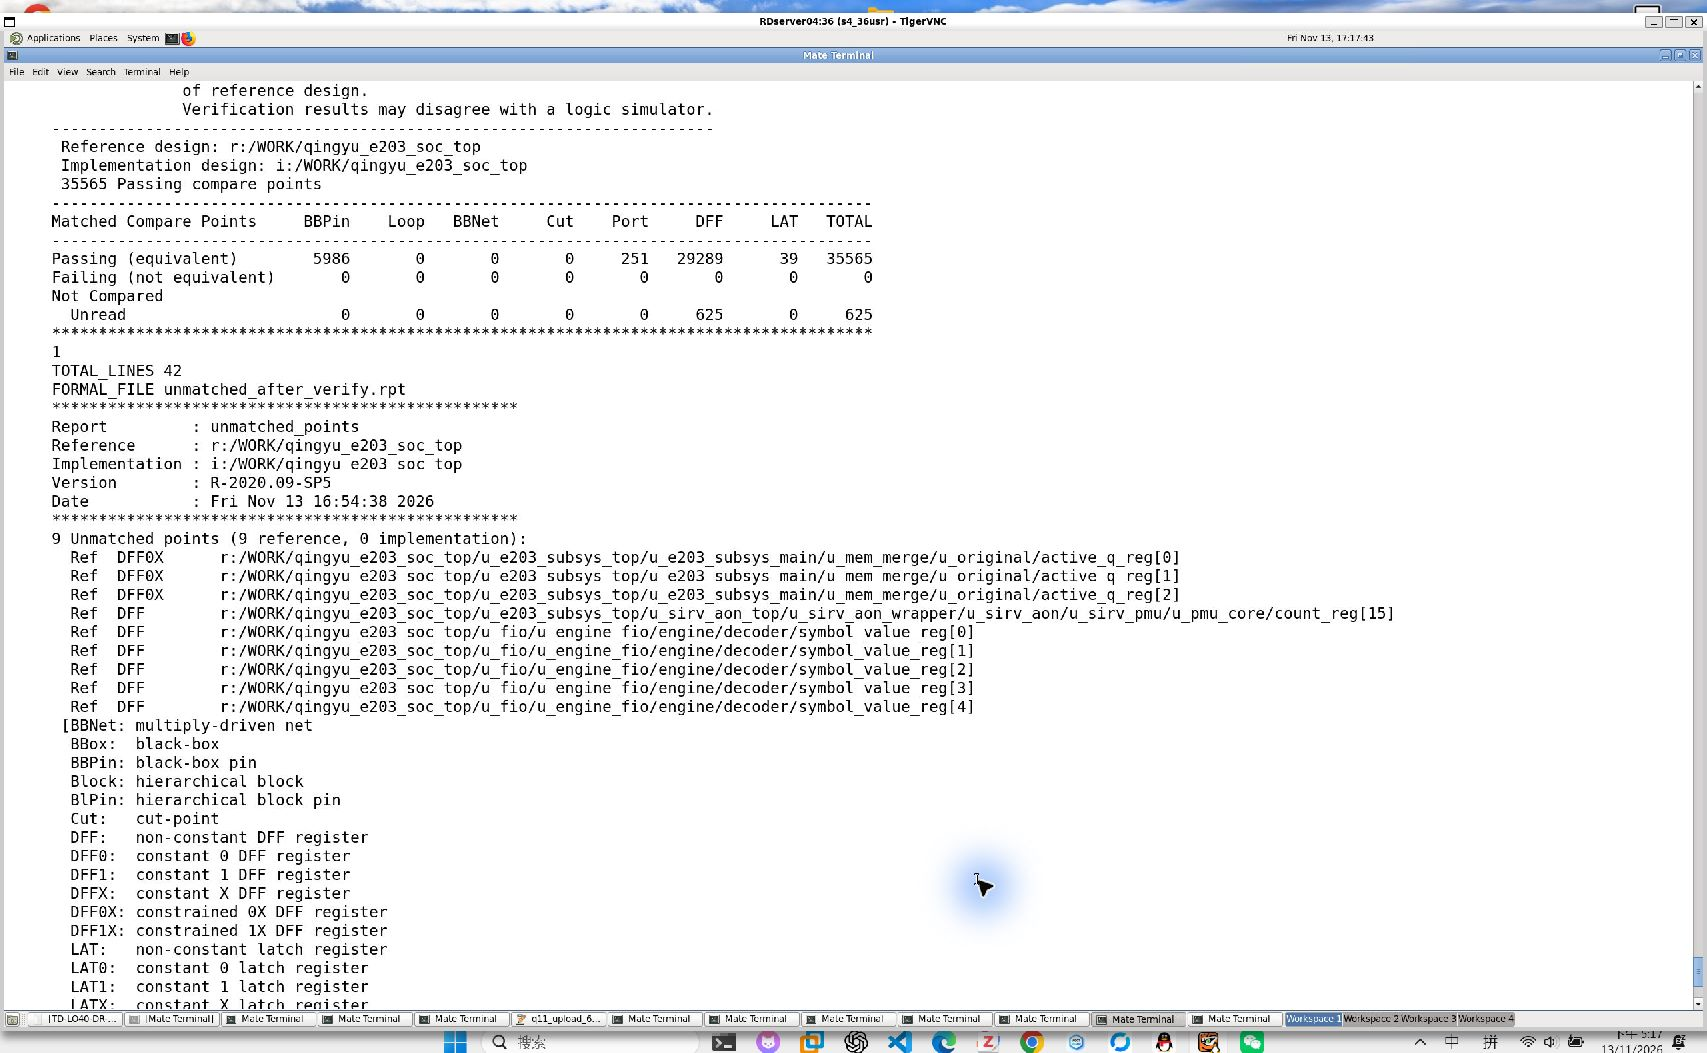
\includegraphics[width=.98\linewidth,height=.80\textheight,keepaspectratio]{assets/27_formal_unmatched_points.png}
\caption{原始记录 E：35565 个通过点、0 个失败点，以及 625 个 unread 点和 9 个参考侧未匹配点。严格等价审计仍未闭合。}
\end{figure}\clearpage
\end{landscape}

\begin{thebibliography}{9}
\addcontentsline{toc}{section}{参考文献}
\bibitem{guide} 全国大学生嵌入式芯片与系统设计竞赛组委会. 芯片设计赛道赛题指南：正式赛题. 2026，15 页.
\bibitem{qa} 全国大学生嵌入式芯片与系统设计竞赛组委会. 芯片设计赛道赛题问题答复. 2026，4 页.
\bibitem{upload} 全国大学生嵌入式芯片与系统设计竞赛. 芯片设计赛道作品上传要求（初赛）. 2026.
\bibitem{hbird} E203 hbirdv2 开源处理器工程. 随本设计归档的 RTL 与 LICENSE，参见冻结工程 \path{src/vendor/e203_hbirdv2/}.
\bibitem{source} 轻语项目. Q12 native12 earlycheck 冻结源码与证据. 2026-11-13. 标签 \code{q12-submission-20261113-r1}，提交 \code{8731bf4}.
\bibitem{eda} 轻语项目. 同版 DC、Formality、PrimeTime 原始报告及 VNC 记录. 2026-11-13，授权服务器工程留存；本报告列出源与网表身份.
\end{thebibliography}
\end{document}
